\resetdatestamp

\chapter{Vizmapper}

With the benefit of the research and context that is presented in chapters 2 and 3, it is now possible to embark on an informed analysis of the mapping task for an MSN and to make informed decisions about the implementation of the system.

The graphical user interface to Libmapper that is the result of these design choices is called Vizmapper.

The task of mapping is understood, from chapter 2, to be creating a set of associations and functional transformations between a set of signals being output by a set of devices (usually with sensors) and a set of inputs made available by various devices (usually with audio synthesis modules)  capable of receiving signals.

The context for the mapping task is understood to be one where many programmers, engineers, composers, and/or musicians are interested in experimenting with interactive musical systems for use in a creative (as opposed to productivity or analysis) context.

\section{Task Analysis of DMI Mapping}
\begin{comment}
Task analysis and human-computer interaction: approaches, techniques, and levels of analysis - Abe Crystal, Beth Ellington
\end{comment}

The section on task analysis in chapter 3 concluded that, as a technique, it is best-suited to understanding how to design interfaces that maximize productivity as opposed to channeling creative expression. This may or may not present a problem depending on whether we choose the characterize the use of computers, in the context of accomplishing the task of mapping, as an act of expression or an act of productivity. Atau Tanaka offers a line of thinking that applies to tools and instruments, but may be of use in attempting to resolve this problem \cite{tanaka2000}.

\begin{quote}
"A tool can be improved to be more efficient, can take on new features to help in realizing its task, and can even take on other, new tasks not part of the original design specification. In the ideal case, a tool expands the limits of what it can do. It should be easy to use, and be accessible to [sic] wide range of naive users. Limitations or defaults are seen as aspects that can be improved upon.

A musical instrument's raison-d'etre, on the other hand, is not at all utilitarian. It is not meant to carry out a single defined task as a tool is. Instead, a musical instrument often changes context, withstanding changes of musical style played on it while maintaining its identity. A tool gets better as it attains perfection in realizing its tasks. The evolution of an instrument is less driven by practical concerns, and is motivated instead by the quality of sound the instrument produces. In this regard, it is not so necessary for an instrument to be perfect as much as it is important for it to display distinguishing characteristics, or "personality". What might be considered imperfections or limitations from the perspective of tool design often contribute to a "personality" of a musical instrument.

Computers are generalist machines with which tools are programmed. By itself, a computer is a tabula rasa, full of potential, but without specific inherent orientation. Software applications endow the computer with specific capabilities. It is with such a machine that we seek to create instruments with which we can establish a profound musical rapport.

The input device is the gateway through which the user accesses the computer software's functionality. As a generalist device, generalized input devices like the keyboard or mouse allow the manipulation of a variety of different software tools. Music software can be written to give musically specific capabilities to the computer. Input devices can be built to exploit the specific capabilities of this software. On this general platform, then, we begin to build a specialized system, each component becoming part of the total instrument description." 
\end{quote}

This line of thinking suggests that the extent to which Vizmapper is not a tool limits the extent to which the principles of user interface and data visualization design ought to play a role in the design process. HCI is much better suited to evaluating more objective notions like utility, tasks, and functionality than more subjective notions like personality, quality of sound, and musical rapport.

It is clear from Tanaka's definitions that Vizmapper serves as a tool rather than an instrument. However, the fact that Vizmapper is specifically a tool for accomplishing the task of creating and modifying mappings \emph{within a musical instrument} suggests that the design must be treated more subtly in this particular context. As the purpose of Vizmapper is partly to make the connections between components in a musical instrument more malleable and more susceptible to experimentation for groups of non-programmers, the task bears some resemblance to a non-utilitarian task. It is reasonable to assume that if the evolution of an instrument is motivated by the quality of the sound that the instrument produces, then similarly the evolution of a mapping interface is motivated by the quality of the mappings and DMIs that the interface produces. This reality should be evaluated in parallel with the understanding that configuration of a mapping is a somewhat utilitarian task; either the interface allows a team to configure the mapping efficiently or it does not.

To see this, the complex task of designing a musical instrument is deconstructed using an analysis process called \emph{hierarchical task analysis} \cite{annett1967}. 

Wanderley and Depalle nicely distill the last decade of thinking into understanding the abstract components of a digital musical instruments by decomposing a digital musical instrument into 3 main components \cite{wanderley2004}:

\begin{description}
\item \emph{The physical interface} containing the sensors, actuators, and physical body of the instrument.
\item \emph{The software synthesis system} which creates both the sonic output of the instrument and any visual, haptic and/or vibrotactile feedback.
\item \emph{The mapping system} in which connections are made between parameters of the physical interface and those of the synthesis system.
\end{description}

The design of these 3 components can be regarded as the 3 main subtasks of the overall task of designing a digital musical instrument. Each of these subtasks are themselves composed of more granular tasks, thus forming the beginnings of a hierarchical structure representing an analysis of the overall task.

\begin{description}
\item \emph{Designing the physical interface}
\begin{description}
\item choose sensors that are capable of detecting the desired physical phenomena or gestures
\item choose actuators that are capable of inducing the desired physical phenomena or feedback
\item choose sensors that are made available as outputs for connections to the inputs of the synthesis system
\item choose actuators that are made available as inputs for connections from the outputs of the synthesis system
\item choose structural/aesthetic materials that combined with the sensors and actuators will form the composite form of the physical interface
\item design the shape, look, feel of the composite physical interface
\end{description}
\item \emph{Designing the software audio synthesis system}
\begin{description}
\item choose a mechanism/algorithm for performing sound synthesis in software
\item choose a mechanism/algorithm for generating visual, haptic, and/or vibrotactile feedback
\item choose parameters of sound synthesis that are made available as inputs for connections from the outputs of the physical interface and/or other components of the composite synthesis system
\item choose parameters of visual, haptic, and/or vibrotactile feedback synthesis that are made available as inputs for connections from the outputs of the physical interface and/or other components of the composite synthesis system
\item choose parameters of sound, visual, haptic, and/or vibrotactile synthesis that are made available as outputs for connections to the physical interface and/or other components of the synthesis system
\end{description}
\item \emph{Designing the mapping}
\begin{description}
	\item choose a subset from the complete set of available outputs to start connections from
	\item choose a subset from the complete set of available inputs to connect to specific outputs
	\item create functional transformation mappings that specify how (if at all) to modify source signals from outputs to generate the desired destination signals for the inputs
\end{description}
\end{description}

This hierarchical model of musical instrument design generalizes well to anything from a self-contained handheld instrument to a massively distributed system spread over a large physical environment. It also works regardless of whether it is an individual or a team that is engaged in the instrument design. This decomposition also makes more clear why perhaps the mapping system is deserving of a dedicated system and user interface to manipulate. 

A good analogy is the choice of what collection of LEGO blocks to use as opposed to how to put the LEGO blocks together once the blocks are chosen. Procedurally, one chooses what types of blocks to use before deciding how to put the blocks together. Similarly, it makes sense to make certain choices about what pieces will be used for the physical interface and the software synthesis system before deciding how the mapping system will put the two collections of inputs/outputs together. It is difficult to map between two sets of signals when the sets of signals are not already defined. Of course, this model laying out the necessary choices to be made says nothing about \emph{what} choices should be made. That process is entirely dependent on the artistic intentions of the design team and the goal of a mapping tool is only to allow the choices that are made in the mapping subtask to be implemented as efficiently as possible.

\section{Implementation}

As a piece of software, there are a limited number of options for implementing the system while ensuring that the system can be reliably used on the variety of systems that a team designing a musical system is likely to be using in the present and future. As of the time that this system has been implemented, the most common form factors for computers are desktops, laptops, tablets, and smartphones. Each form factor is typically loaded with one of a small collection of operating systems that are widely available and easy to find expert knowledge about.

\begin{description}
\item[Desktops/Laptops] Windows (XP, Vista, 7), Mac OSX, Linux (Ubuntu, Debian, etc.)
\item[Tablets/Smartphones] Android, iOS
\end{description}

This is not an exhaustive list, however the point is that it is not practical (especially in a research context) to develop and maintain several versions of a software system that will work on a wide variety of operating systems and devices. However, the fact is that people will use whatever system they have available and the variety of devices that an artist or engineer is likely to use to interact with a sensor network is increasing. To design a practical system that is meant to work in a collaborative context, it is crucial to adapt to this reality.

Before beginning development on a software system, it is necessary to choose a development environment and a deployment environment. There are any number of very stable development environments that enable a software developer to write a single collection of programmer code and translate the code into executables that can run on Windows, OSX, and Linux machines. These choices effect the developer of the software and not the user of the software. The choice of deployment environment is much more consequential to the user because it effects how they will actually run the executable. For an explaination of technical terms pertaining to this chapter review the appendix.

There are three common methods for a user to run software on their chosen machine.

\begin{enumerate}
\item The first method is for the user to run a compiled machine code executable, which means that the developer has written code and translated the code with a compiler into machine code that can be executed without any further translation on the user's specific machine and operating system. If there is no available compiled executable for a specific machine architecture, the user can obtain the programmer code and compile it into an executable that works on their specific machine as long as a compiler exists for their machine. This is how many video games are deployed.

\item The first method is an option when the software is developed in a \emph{compiled language} environment. There are also environments that use \emph{interpreted languages} or \emph{script languages}. An interpreted language differs from a compiled language because unlike a compiled language that uses the process of translating the program code into machine code with a compiler and producing a machine code executable to run the program, an interpreted language uses the process of interpreting the program code line by line directly when the program is run. The interpreter is responsible for interfacing with the machine for the interpreted code when the executable is run. In a interpreted language the programmer code and the executable are often the same file. Conversely, a compiled executable interfaces directly with the machine because it has already been converted into machine code. 

A web application is essentially an interpreted executable because a web browser that runs HTML, CSS, and Javascript downloads the programmer code and uses an internal interpreter to execute the program. It does not download a compiled executable. Distributing software as an interpreted script executable to be run in an interpreter is attractive because the burden for implementing the interpreter for various different machine architectures is moved to the developer of the programming language and the developer can count on a user being able to run their program as long as the interpreter for the language is available for the user's machine. The developer can write \emph{machine-independent} code.

\item Environments like Java use a third strategy and run software on \emph{virtual machines}. A virtual machine language is somewhat like a hybrid of a compiled language and interpreted language because a virtual machine language is compiled, but it is compiled to an intermediate machine code that is not the machine code of the actual physical machine that is running the program. It is compiled to the "machine code" of a software virtual machine that must be implemented for all machines that one would like to run the program on. This is useful because the user can be given a single file that is not programmer code like a script executable, but the developer can still count on the file being able to run on any machine that has the virtual machine available on the system.
\end{enumerate}

Assuming the intent is for multiple team members to be running the Vizmapper interface to enable simultaneous work on the mapping of a network and that there is presumably a local network available to allow the various devices on the sensor network to communicate with each other, suggests Vizmapper ought to be implemented as a web application. 

A web application is typically distributed as a two part software system where one part is called the \emph{client} and the other part is called the \emph{server}. One server can serve the web application to a large number of clients. This is the source of another advantage of web applications. A web client runs in a web browser and therefore can be run on any machine that includes a modern web browser, which includes every operating system listed at the beginning of this section. All modern web browsers provide an increasingly identical deployment environment. Since Libmapper is compiled code, the server software can take care of interfacing with the library and communicating through the Mapper Protocol with the rest of the network. Despite the fact that the server is more restricted as to what deployment environment it can be run on because of the Libmapper dependency, the server needs to run on only one machine. Also, a web application is much easier to deploy on a collection of heterogenous machines. At this point in time, a web client reduces the likelihood that the team will be forced to huddle around the chosen few machines that can run the client, even if all machines cannot run the server with a more restrictive deployment environment.

Stephen Sinclair, the developer of Libmapper and a member of IDMIL, also developed a basic server written in Python (a popular interpreted language) that interfaces with Libmapper and provides a convenient interface for a web browser client to indirectly speak the Mapper Protocol to the local network of devices by communicating with the server. This web server is called Webmapper. Together, Webmapper/Vizmapper provides a server/client web application that can be used to configure a Mapper network.

\section{Application of User Interface Design Principles}
\label{sec:userInterface}

If the user of Vizmapper is a human user configuring an MSN, then Vizmapper is the "user" of Webmapper. Webmapper is then the "user" of Libmapper. Libmapper provides an interface for Webmapper to speak the Mapper Protocol and Webmapper provides an interface for Vizmapper to indirectly speak the Mapper Protocol. Now the task remains to decide how the Vizmapper interface will present the signals and devices present on the network to the human user and allow the user to configure mappings between these signals and devices through Webmapper.

As a reminder, the subtask of \emph{Designing the Mapping} was further broken down as follows:

\begin{description}
	\item choose a collection of available outputs to start connections from
	\item choose a collection of available inputs to connect to specific outputs
	\item create mappings that specify how (if at all) to modify source signals from outputs to generate the desired destination signals for the inputs
\end{description}

From the hierarchical task analysis of designing a DMI, it can be argued that the task of designing a mapping is a less complex task (but not less important) than the task of designing a physical interface or designing an audio synthesis system. This lack of complexity in the task is one of the reasons why it is possible to even contemplate performing the other task through a single interface. Building an interface for the task of designing a physical interface or designing an audio synthesis system is less manageable in this way.

Instead, the complexity of the task lies in the complexity of the Mapper network and what the task of \emph{choosing} actually entails. Since the focus is now on the mapping task, it is helpful to see if it is possible to be even more granular in the hierarchical decomposition of the task. 

\begin{description}
	\item choose a collection of available outputs to start connections from
    \begin{description}
        \item view the complete set of output signals
        \item find an output signal to connect to an input signal
        \item select the output signal
    \end{description}
	\item choose a collection of available inputs to connect to specific outputs
    \begin{description}
        \item view the complete set of input signals
        \item find an input signal to connect to an output signal
        \item select the input signal
    \end{description}
	\item create mappings that specify how (if at all) to modify source signals from outputs to generate the desired destination signals for the inputs
    \begin{description}
        \item define a functional transformation/signal conditioning mapping between the output signal and input signal 
        \item connect the signals
    \end{description}
\end{description}

This clarifies the individual steps implicit in the overall task and suggests how to distribute the steps needed in the interface. Since the screen space on a monitor is limited and the most important data about the Mapper network are the names of the signals and the mappings between them, devoting as much space to the visualization of the signals and their connections is a priority.

The first decision made is to separate the viewing and browsing of the MSN from the editing of mappings. Vizmapper treats these two set of subtasks as two different modes. Entering viewing and browsing mode means that it is not possible to modify the mappings of the signals being browsed. Entering editing mode focusing the view on a subset of signals from the complete set and means that it is not possible to browse the larger set of signals. This decision is made because viewing and browsing does not actually effect the Mapper network, only editing a mapping effects the network. Preventing both modes from being accessed on the same screen makes the conceptual separation between the modes clear and reduces the amount of accidental modifications.

When it comes to viewing and browsing, since the interface is being designed with larger MSNs in mind, there should be a way to filter the complete set of signals to a subset of signals. As discussed in chapter 3, this can be accomplished with pointing and clicking to utilize recognition processes or it can be accomplished by typing to encourage the use of recall processes. Although finding a specific signal through name recognition is less straining then remembering the name of a specific signal and typing it, it is not necessarily a simple decision. In the case where a user has been working with the same Mapper network for an extended period of time, it may become tedious to point, click, and browse their way to a specific signal even though they know the exact name of the signal they are looking for. In this case, the physical process involved to select the signal becomes more consciously cumbersome than the cognitive process involved in recognition or recall.

A single text input box for entering a text matching filter query, occupies very little vertical space and adds functionality that is helpful for this type of user. The user can type in a portion of the complete OSC name of a signal and limit the view to only the signals that match the text in the input box. In order to display the union of more than one text query (show the signals that match the first text query OR second query OR third query, etc.), the user uses a space character to delimit the separate filter queries. 

Typically, interfaces that allow the user to browse data using text queries allow the user to compose more complex queries (like ANDs or NOTs in addition to ORs). However, this functionality seems to deviate from the scope of the interface and add syntax complexity without a substantial benefit to the central task. Since the user is only searching within a set names of signals and not a set of large text documents (like one might do with a database or the internet) it is likely a type of power that is not required for most users. Additional features and complexity are avoided in Vizmapper, unless the functionality that is added is significant to the mapping task as it has been analyzed.

\section{Application of Data Visualization Design Principles}

Following the graphical perception research in section \ref{sec:Graphical Perception} of chapter 3, before making decisions about the visualization of the network the data set of a Mapper network needs to be analyzed using the three stage process of Bertin \cite{semiology1983}.

This involves determining the \emph{components} in the data, the \emph{length} of each component, and the \emph{level of organization} (nominal, ordinal, or quantitative).

There are three easily distinguishable sets of data that a user concerns themselves with when mapping signals.

\begin{enumerate}
\item set of signals on the Mapper network, which are defined as OSC names that are part of a hierarchical namespace
\item set of associative connections between pairs of signals, each connection is defined by a source and a destination (the source of the data is typically an output signal and the destination is typically an input signal)
\item set of function transformations that are paired with each associative connection, which are defined using a function type, a mathematical function, and an allowable range of values for the input of the function (actually an output signal in Mapper terminology) and output of the function (actually an input signal in Mapper terminology)
\end{enumerate}

It is useful to note that the most complex elements are the elements of the set of functional transformations. The least complex elements are the OSC names of the signals. This is taken simply from the number of variables that must be defined to fully define each element.

So the data set can be decomposed into \emph{three} components, but it might also be decomposed into \emph{four}. The first component, the set of signals, can be split into one component for output signals and one component for input signals. The question is whether one decomposition is more effective than the other. If it is assumed that the source of a connection will always be an output signal of a device and the destination of a connection will always be an input signal of a device then it makes sense to use \emph{four} because it will always be necessary to select a source and a destination to form any connection and it will be efficient to graphically distinguish between the two types of signal. Therefore, there are \emph{four} components in the data set. The first component of the previous decomposition can be further split into:

\begin{enumerate}
\item set of output signals on the Mapper network, which are defined as OSC names that are part of a hierarchical namespace
\item set of input signals on the Mapper network, which are defined as OSC names that are part of a hierarchical namespace
\end{enumerate}

The length of the output signals component and the input signals component are assumed to be \emph{large} and within an order of magnitude of each other. There might be many more output signals than input signals or vice versa, however since there will be roughly one control mechanism device with output signals for each sound generation mechanism device with input signals in a scenario with DMIs, this is a reasonable assumption.

The length of the set of associative connections is bounded by the length of the set of output signals. This is because the Mapper protocol only handles \emph{one-to-many} and \emph{one-to-one} mappings as explained in chapter 2. Therefore, there can be at most one connection for every output signal.

The length of the set of function transformations is equal to the length of the set of associative connections because every connection is paired with a functional transformation governing data transmission over the connection. This is not strictly true, however it is simpler to treat those connections with no active transformation as utilizing the function of \begin{math}x = y\end{math} to indicate the lack of any signal conditioning.  

The level of organization of all four components is \emph{nominal}. None of the components have elements that can be ordered or manipulated with arithmetic.

So the conclusion of a Bertin-like analysis of a typical Mapper network data set is the following:
\begin{description}
\item \emph{Components} - four components
    \begin{enumerate}
        \item output signals
        \item input signals
        \item connections
        \item functional transformations
    \end{enumerate}
\item \emph{Length} - all four components are of approximately equivalent length
\item \emph{Level of organization} - all four components are nominal
\end{description}

This analysis comes with one caveat in light of chapters 2 and 3. There is one level of organization that Bertin does not address - hierarchical organization. This is a type of organization that seems relevant, especially given the importance of hierarchical organization in human cognition, yet seems to not be directly addressed by the nominal/ordinal/quantitative categorization scheme. Due to the nature of OSC namespaces, the set of output signals and the set of input signals can be grouped hierarchically. This suggests a type of relation between signals that is not simply = or NOT =.

The problem of visualizing an abstract data set that has both hierarchical relationships between elements and connections between elements as components is problem that has been tackled in data visualization literature \cite{edgebundles2006}. Holten refers the hierarchically organized component as a set of \emph{inclusion relations} and the set of connections as a set of \emph{adjacency relations}. One example of a data set exhibiting a structure similar to a Mapper network data set is an academic citation network where publications are the lowest level elements of the hierarchy and departments and universities are represented by higher level groupings in the hierarchy. Connections between publications would represent one publication citing another \cite{edgebundles2006}.

Since we are dealing with nominal data with some hierarchical organization, let us focus on the most discerning perceptual tasks for nominal data using the ranking presented in section \ref{sec:Graphical Perception}.

\begin{table}
    \begin{center}
    \begin{tabular}{ | l | }
    \hline
    Nominal \\ \hline
    Position \\
    Color Hue \\
    Texture \\
    Connection \\
    Containment \\
    Density \\
    \hline
    \end{tabular}
    \end{center}
    \caption{Ranking of top perceptual tasks for discerning between nominal data \cite{jock1986}}
    \label{tab:perceptualNominal}
\end{table}

Inspired by Holten's own exploration of visualizing similarly structured data, the decision is made to represent signals with circles occupying different points in space. The heuristic reasons for this decision is that the shape of a circle lends itself to a symmetrical and aesthetically pleasing presentation of the data and makes for an easy target for the user to click (more on this shortly). There are four components and it is important to distinguish between these four components, first and foremost. Since position is already being used to distinguish between signals and at least one output signal and one input signal will need to be displayed for the connection and functional transformation components to be relevant, it makes sense to place a constraint on the \emph{position} of signals that forces the output signals to be confined to the left side of the display and input signals to be confined to the right.

\begin{figure}[htb]
\centering
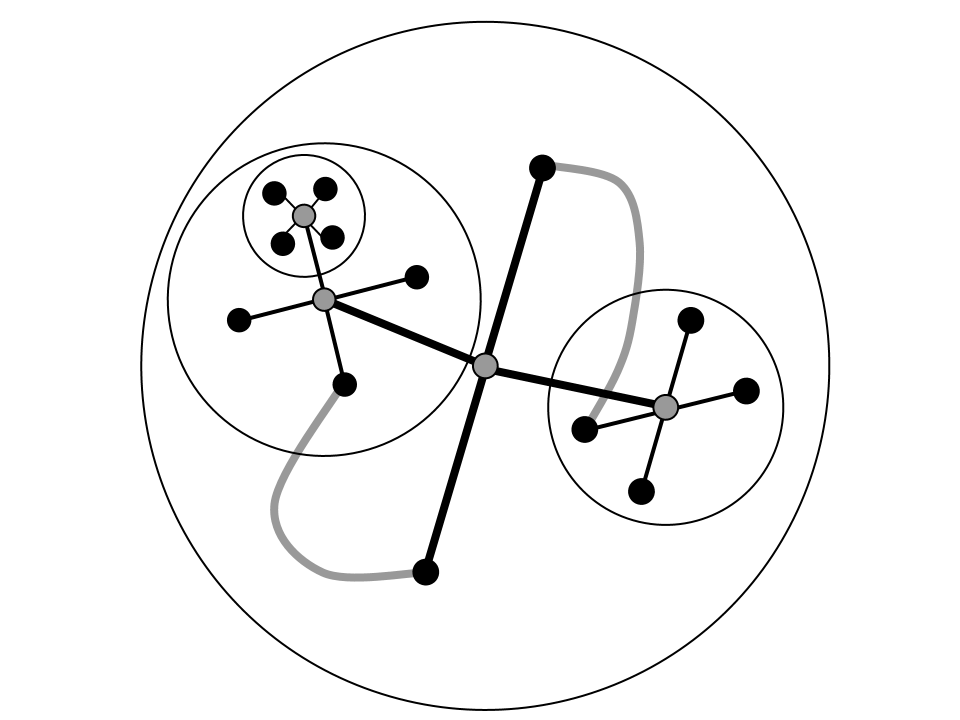
\includegraphics[width=0.6\textwidth]{holten_balloon.png}
\caption{Example of a balloon tree visualization with dark lines for inclusion relations and light lines for the adjacency relations - inspired by \cite{edgebundles2006}}
\label{fig:balloonTree}
\end{figure}

The decision is made to use containment to represent the inclusion relations between hierarchically organized elements. This is taken from the use of a \emph{balloon tree} visualization by Holten in his own research. An example of a balloon tree is shown in Figure \ref{fig:balloonTree}. Examining the figure, notice that \emph{connection}, \emph{containment}, and \emph{density} are used to communicate specific relationships between elements. Again, there are two components being displayed: a set of inclusion relations and a set of adjacency relations. In this example there are only two adjacency relations shown in the figure. 

Connection is used to communicate both adjacency and inclusion. The curved, lighter lines represent adjacency relations between terminal elements (for example, citations between publications). The straight, dark lines represent inclusion relations between different levels in the hierarchy. Density and shape are used to distinguish between the two. Density is also used to distinguish between terminal elements in the hierarchy (dark dots) and intermediate elements in the hierarchy (light dots, for example, representing departments and universities). 

Containment and position are also used to communicate relations between the elements. Enclosing circles differentiate between levels in the hierarchy and different branches of the hierarchy on the same level. The center of every circle is the position of the intermediate elements defining what the circle represents (for example, department on one level of hierarchy, university on another level) and the elements positioned radially around the centers are the child elements (either terminal or lower level, but still intermediate, elements). Notice that terminal elements can either be placed directly on the first level of the hierarchy or on deeper levels depending on the specific inclusion relations of the data set (perhaps there are independent publications that are not associated with any particular organization in the data set).

\begin{figure}[htb]
\centering
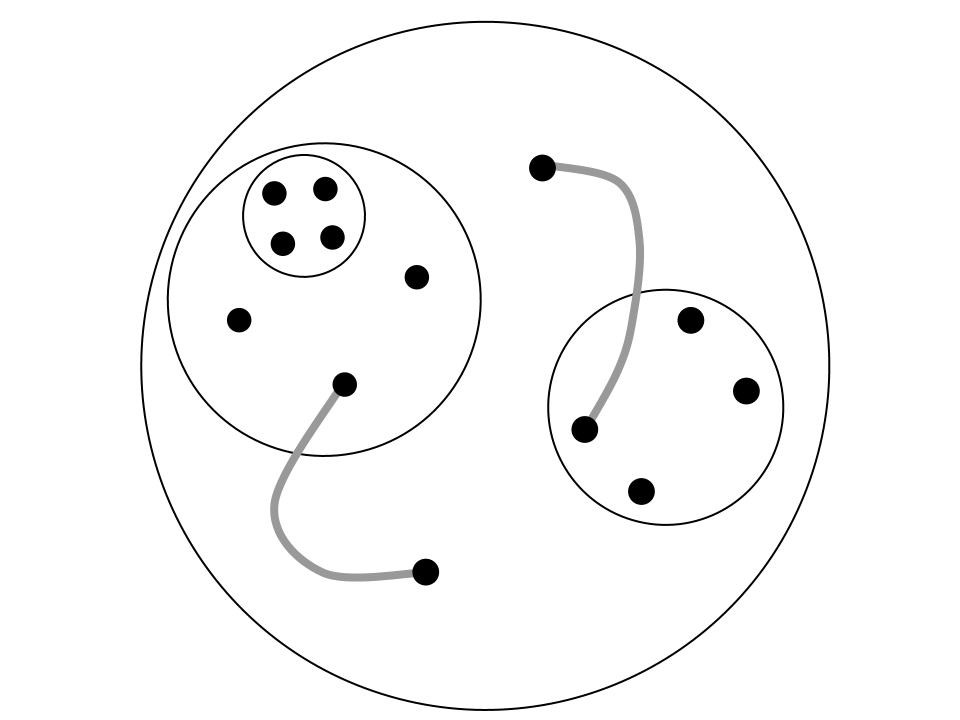
\includegraphics[width=0.55\textwidth]{vijay_balloon.png}
\caption{Modified balloon tree visualization}
\label{fig:balloon}
\end{figure}

The balloon tree used in Figure \ref{fig:balloonTree} is not as uncluttered as it might be. The lines used to communicate inclusion relations and the lighter dots placed at the center of every circle actually display the same data as the containing circles. This seems to be unnecessary visual redundancy. Figure \ref{fig:balloon} effectively communicates the same data set as \ref{fig:balloonTree} with no loss of information and less clutter. The missing visual elements are implied.

\begin{figure}[htb]
\centering
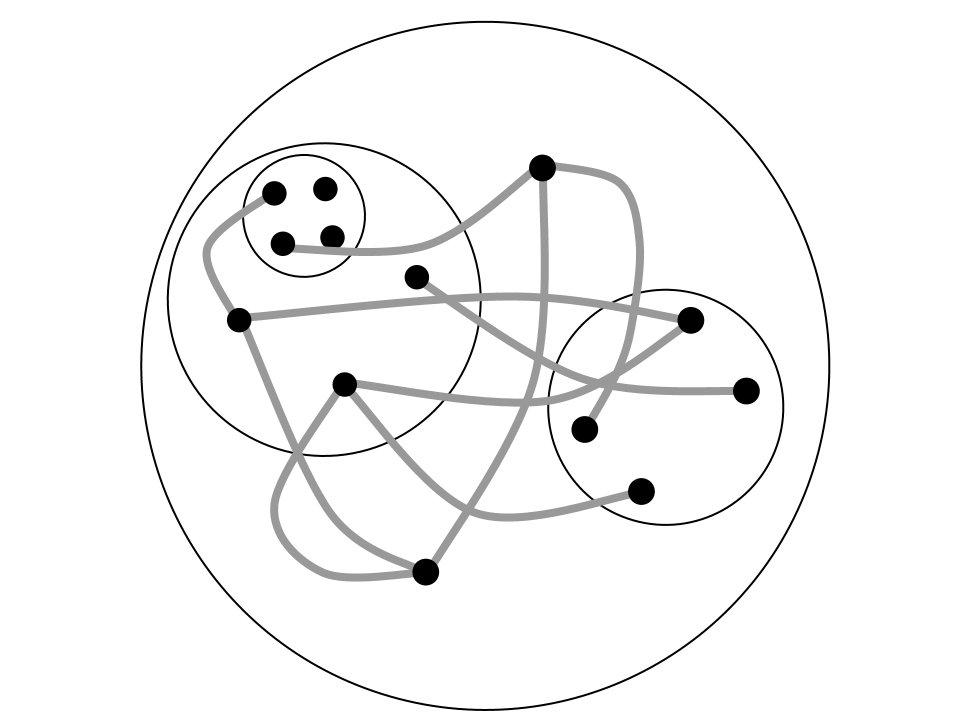
\includegraphics[width=0.55\textwidth]{clutter_balloon.png}
\caption{Cluttered balloon tree visualization}
\label{fig:clutterBalloon}
\end{figure}

When the number of elements in the data set grows large and there are many adjacency relations between the elements, there is a different type of clutter that arises involving the lines representing the adjacency relations like in Figure \ref{fig:clutterBalloon}. This is a type of clutter that is more difficult to reduce. One can be more specific about how the connnections are drawn, using bezier curves and bundling to organize the connections like one might bundle wires between mixers. This is the method that Holten uses \cite{edgebundles2006}. 

It may be possible to use a different graphical property entirely. However, it is difficult to conceive of a graphical property that communicates connections between signals better than the graphical property of connection. One potential way out is realizing that there is no need to treat the visualization as static. It is already possible to use a text-matching filter to modify the visualization by typing within the interface as described in Section \ref{sec:userInterface}. Perhaps it would make sense to allow the user to filter the visualization by pointing and clicking as well.

\begin{figure}[htb]
\centering
\subfloat[Top level][Top level]{
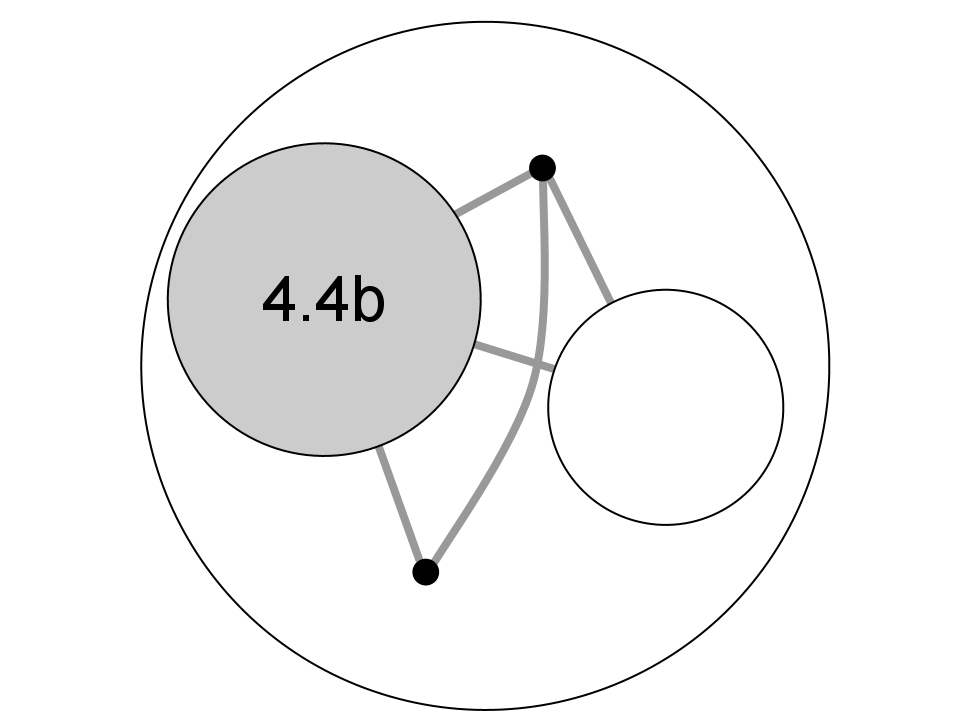
\includegraphics[width=0.33\textwidth]{firstLevelBalloon.png}
\label{fig:unclutteredBalloon}}
\subfloat[Branch of the second level][Branch of the second level]{
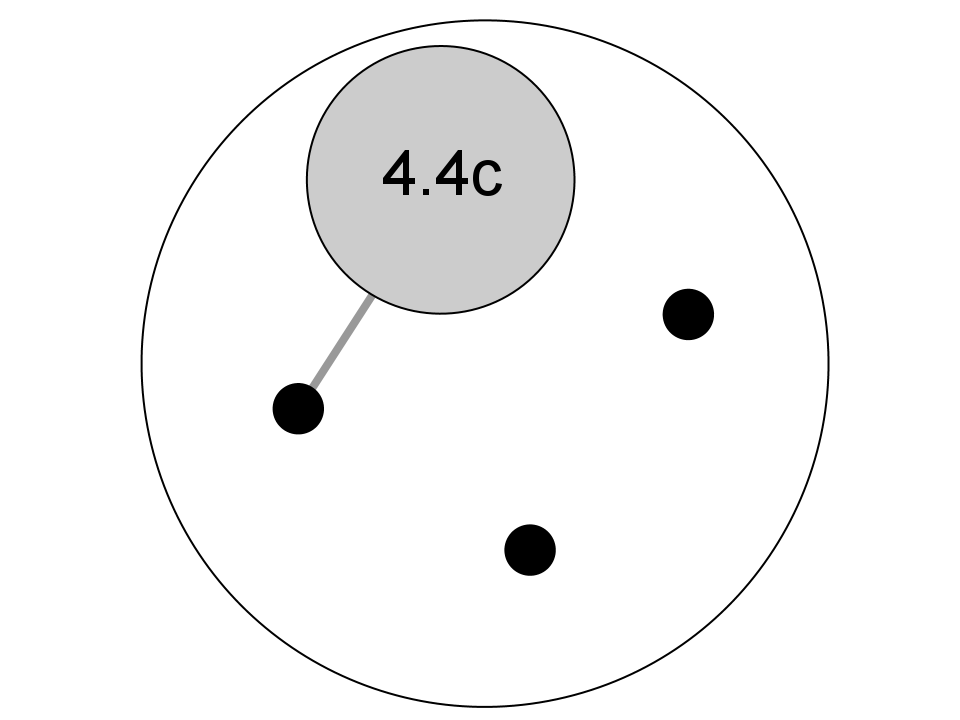
\includegraphics[width=0.33\textwidth]{secondLevelBalloon.png}
\label{fig:secondUnclutteredBalloon}}
\subfloat[Branch on the third level][Branch on the third level]{

\includegraphics[width=0.33\textwidth]{thirdLevelBalloon.png}
\label{fig:thirdUnclutteredBalloon}}
\caption{Interactive balloon tree visualization of hierarchy}
\label{fig:interactiveBalloon}
\end{figure}

In Figure \ref{fig:unclutteredBalloon}, it is clear that it leaves out information present in the other visualizations even though it is supposed to visualize the same data set as the other three figures. However, it displays all the adjacency relations between groups on single level of the hierarchy and displays the inclusion relation between the root of the hierarchy and the first level of the hierarchy. If the user clicks on gray circle in Figure \ref{fig:unclutteredBalloon} representing a branch of the hierarchy on the second level, then the interface can modify the visualization to Figure \ref{fig:secondUnclutteredBalloon}. The user can then click on the gray circle in Figure \ref{fig:secondUnclutteredBalloon} to proceed into the deepest level (which in Figure \ref{fig:clutterBalloon} is the third level) in the whole hierarchy shown in Figure \ref{fig:thirdUnclutteredBalloon}. 

However, this interactive visualization has lost information about the adjacency relations between the current level of the hierarchy and a higher level of the hierarchy. It only displays adjacency relations between the groups on the same level. Therefore, even though Figure \ref{fig:unclutteredBalloon} shows the gray circle having adjacency relations between all the other groups and elements on the top level of the hierarchy, Figure \ref{fig:secondUnclutteredBalloon} loses this information completely and there is no way to recover exactly what terminal elements are connected to each other.

\begin{figure}[htb]
\centering
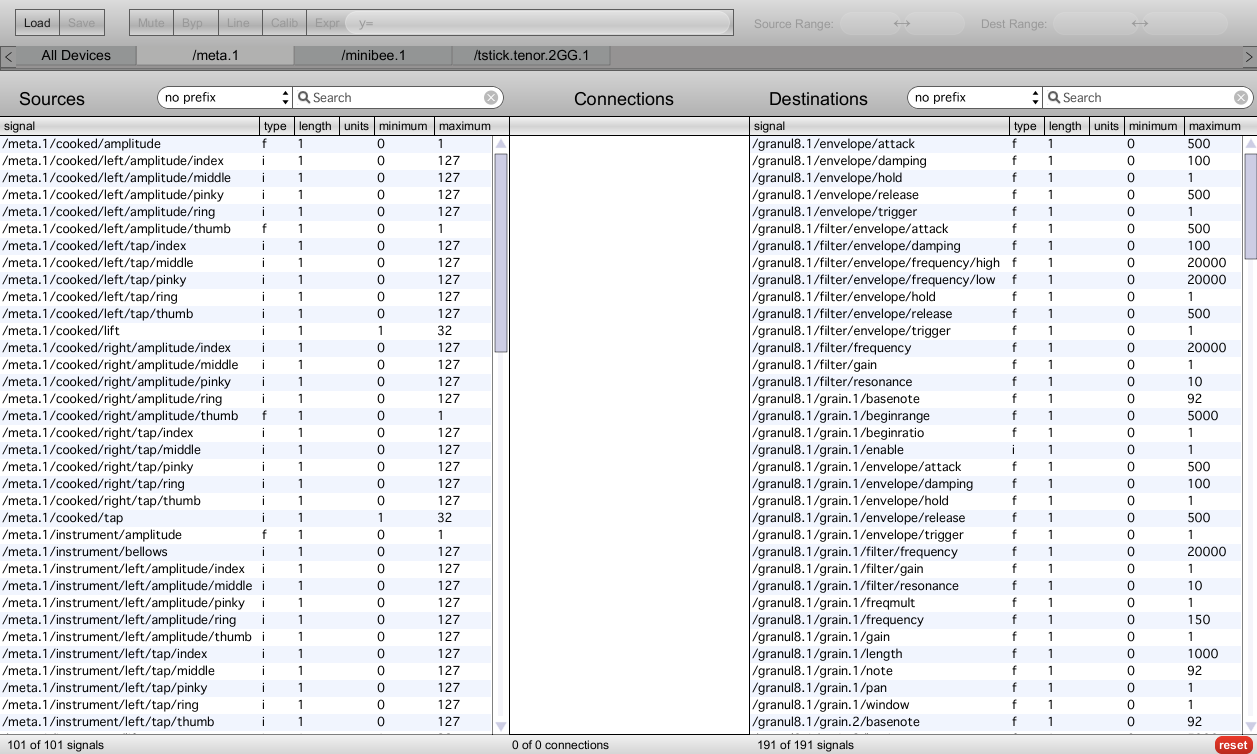
\includegraphics[width=0.88\textwidth]{maxmapperFirst.png}
\caption{/source.3 branch of second level of output signals and /dest.3/synth1 branch of third level of input signals in Vizmapper}
\label{fig:maxOne}
\end{figure}

\begin{figure}[p]
\centering
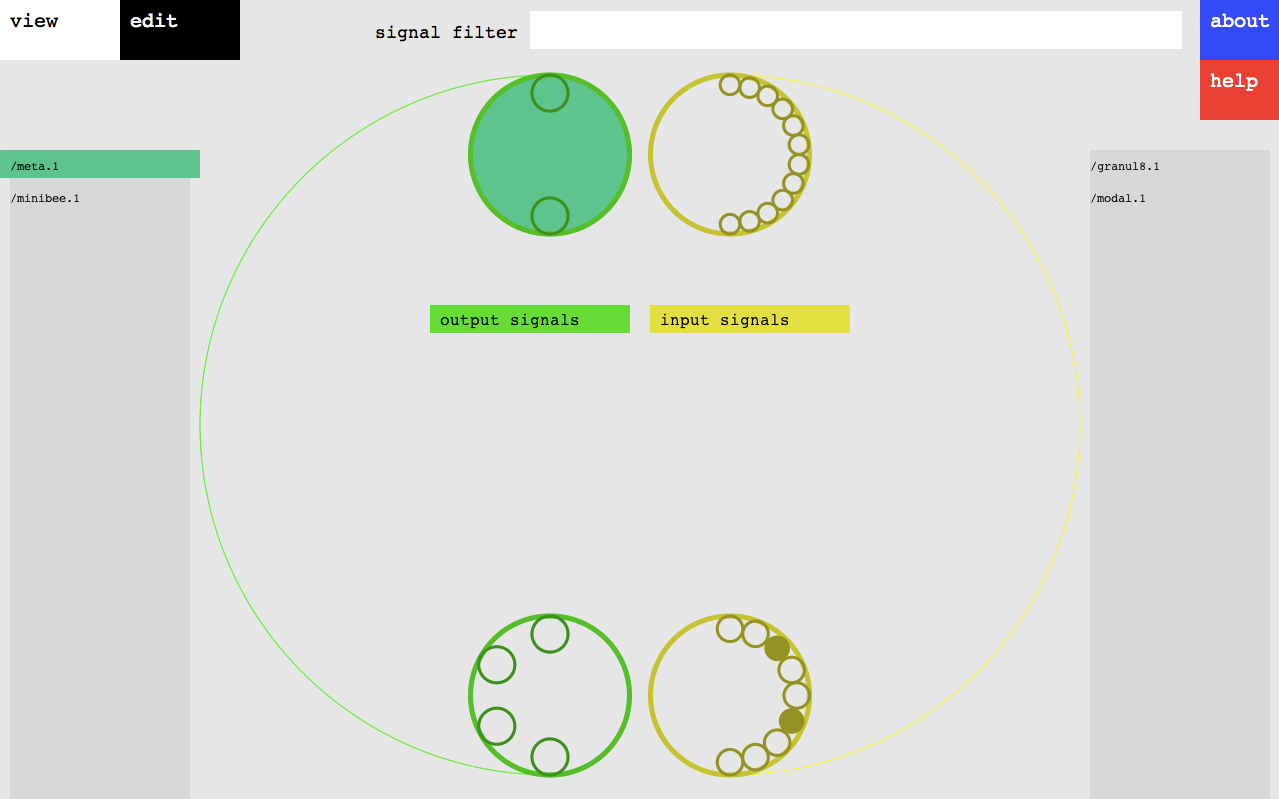
\includegraphics[width=0.88\textwidth]{vizmapperFirst.png}
\caption{First level of output signals and first level of input signals in Vizmapper}
\label{fig:vizOne}
\end{figure}

\begin{figure}[p]
\centering
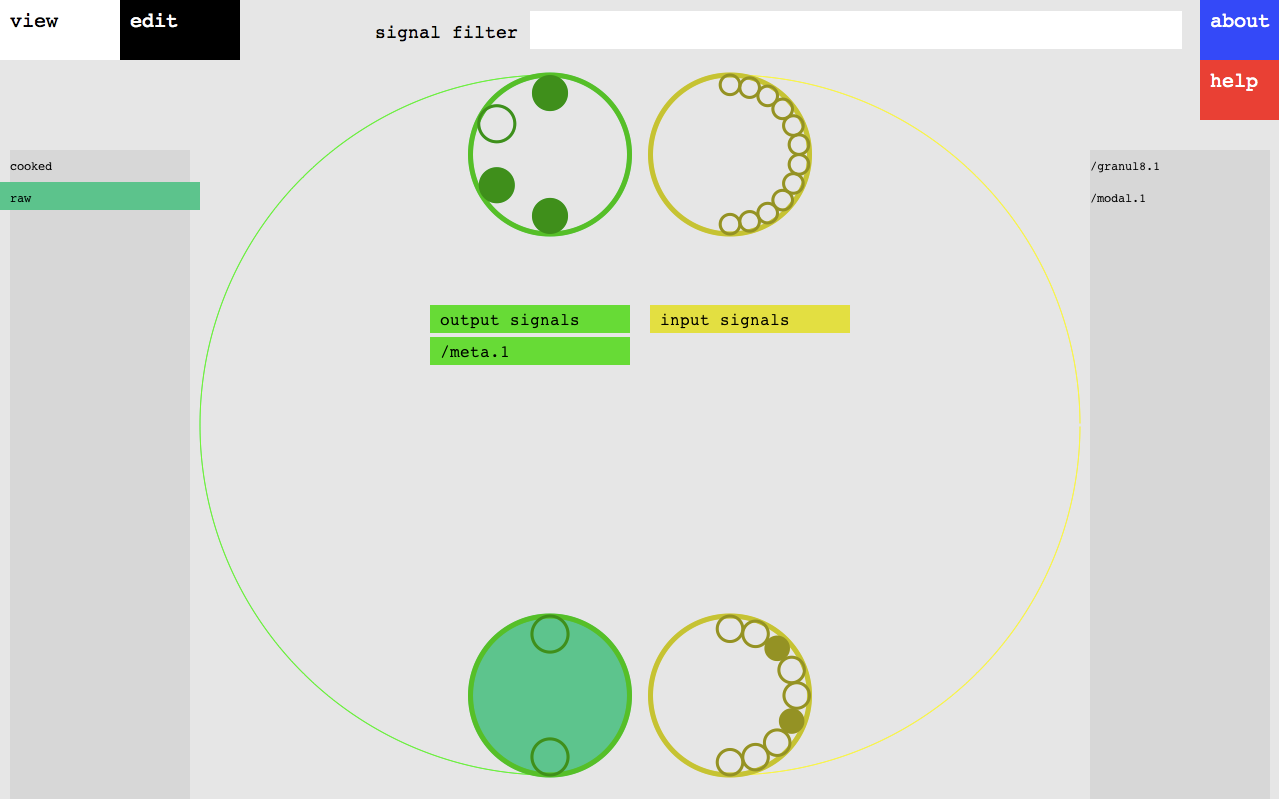
\includegraphics[width=0.88\textwidth]{vizmapperSecond.png}
\caption{/source.3 branch of second level of output signals and first level of input signals in Vizmapper}
\label{fig:vizTwo}
\end{figure}

\begin{figure}[p]
\centering
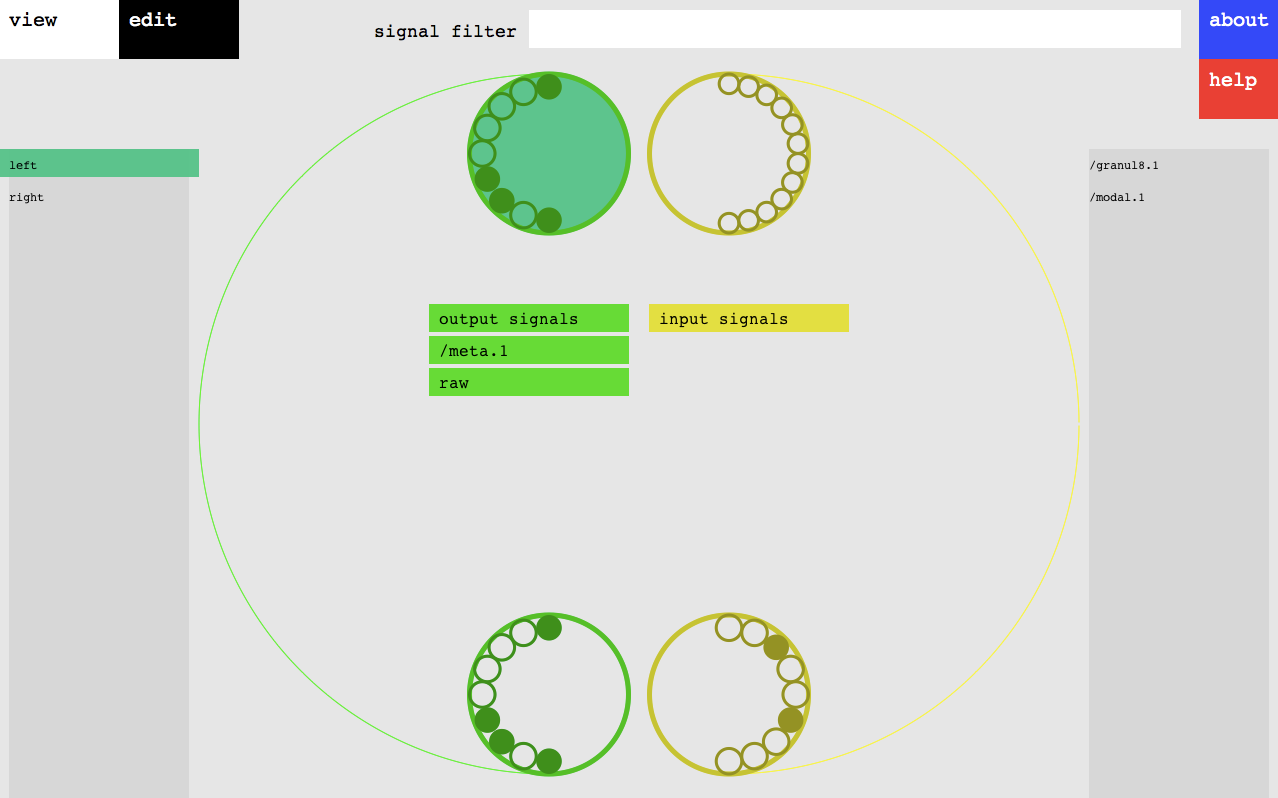
\includegraphics[width=0.88\textwidth]{vizmapperThird.png}
\caption{/source.3 branch of second level of output signals and /dest.3/synth1 branch of third level of input signals in Vizmapper}
\label{fig:vizThree}
\end{figure}

\begin{figure}[p]
\centering
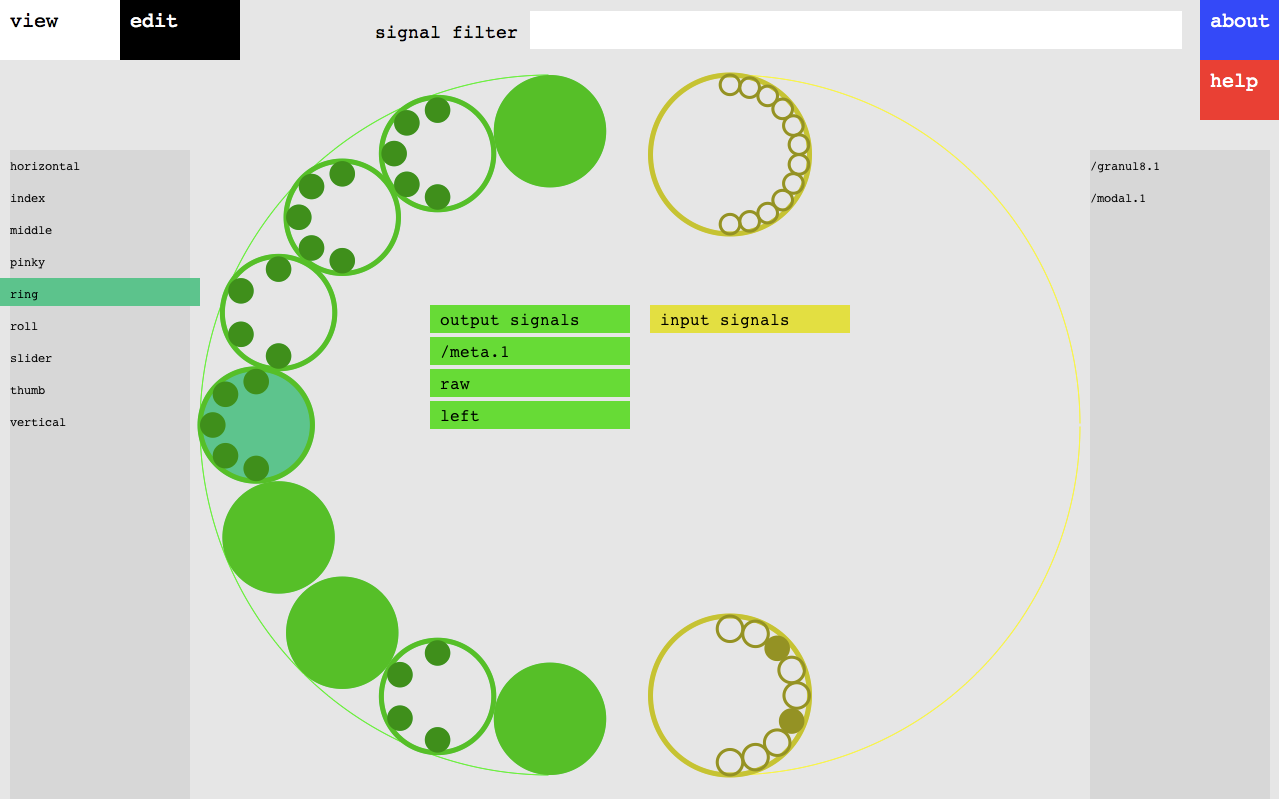
\includegraphics[width=0.88\textwidth]{vizmapperFour.png}
\caption{First level of output signals and first level of input signals in Vizmapper}
\label{fig:vizFour}
\end{figure}

\begin{figure}[htb]
\centering
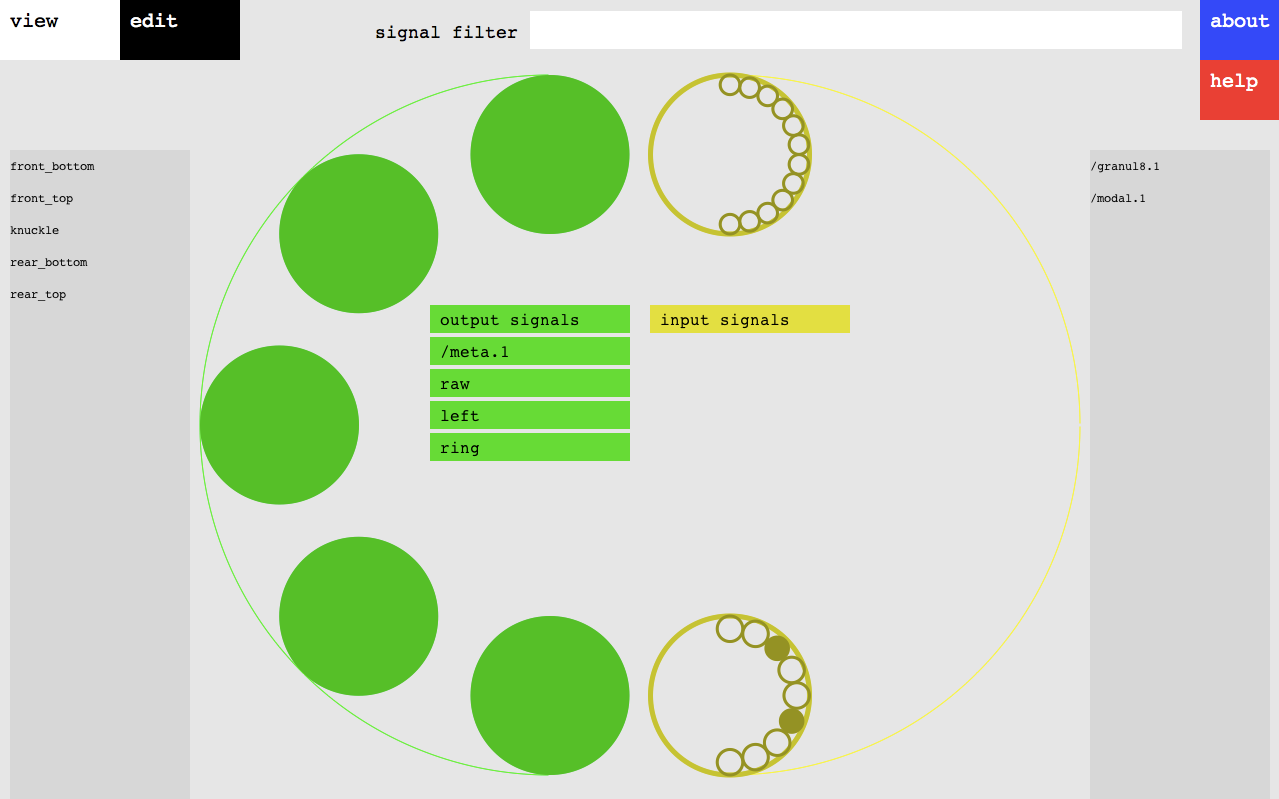
\includegraphics[width=0.88\textwidth]{vizmapperFive.png}
\caption{/source.3 branch of second level of output signals and first level of input signals in Vizmapper}
\label{fig:vizFive}
\end{figure}

\begin{figure}[p]
\centering
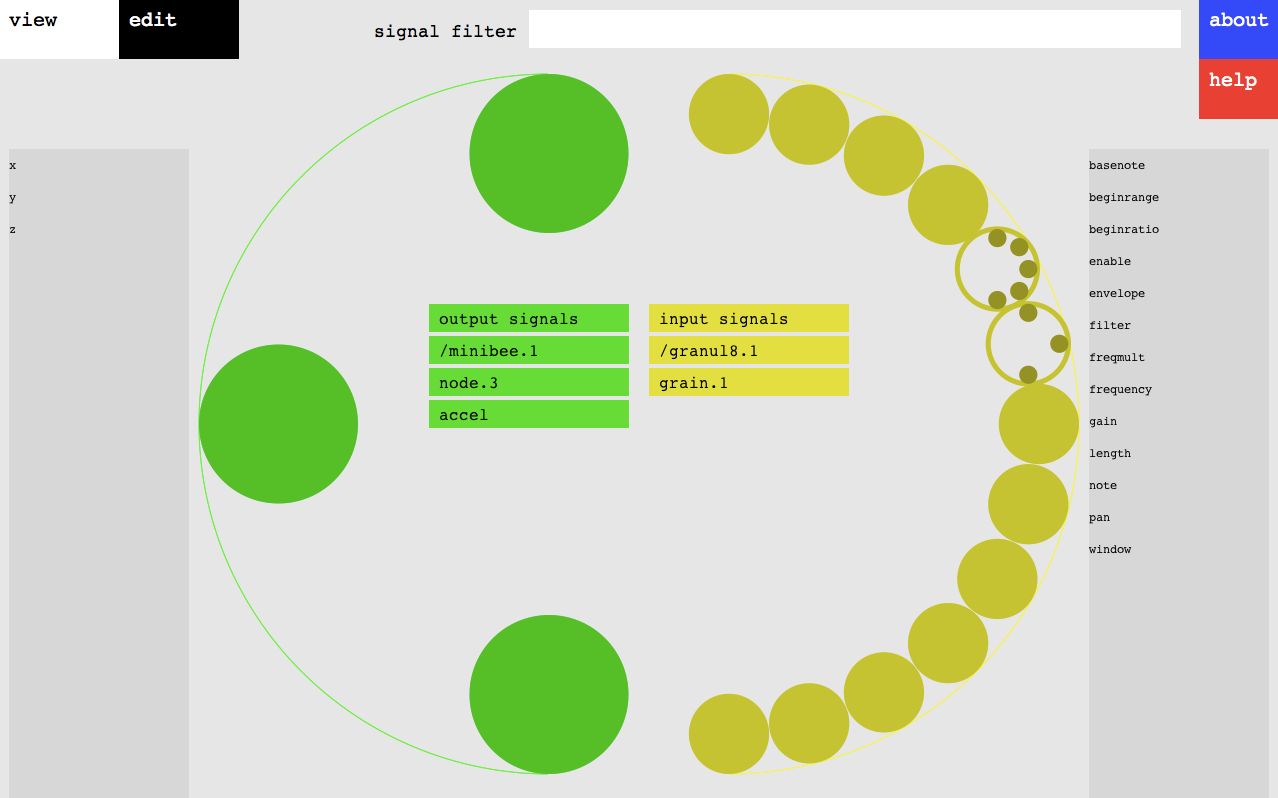
\includegraphics[width=0.88\textwidth]{vizmapperSix.png}
\caption{/source.3 branch of second level of output signals and /dest.3/synth1 branch of third level of input signals in Vizmapper}
\label{fig:vizSix}
\end{figure}

\begin{figure}[p]
\centering
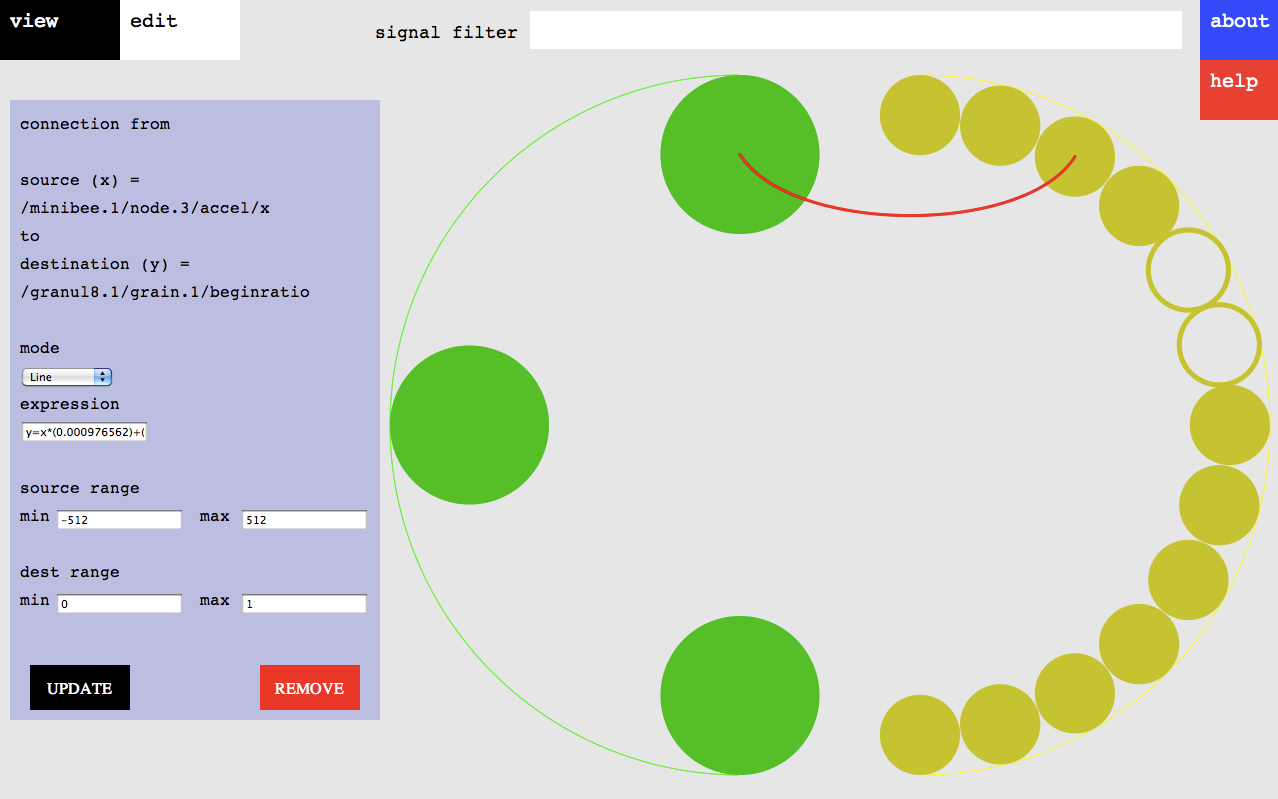
\includegraphics[width=0.88\textwidth]{vizmapperSeven.png}
\caption{First level of output signals and first level of input signals in Vizmapper}
\label{fig:vizSeven}
\end{figure}

Fortunately, a decision made in Section \ref{sec:userInterface} allows this problem to be circumvented. The problem of lost information in this scenario is a result of all of the elements belonging to the same component. Since the decision is made in Vizmapper to separate the potential sources of a connection from the potention destinations of a connection and any given signal can only be an output (source) or input (destination) then this problem is nonexistent.

\section{Vizmapper}

The best way to see how this is to see the visualization used in Vizmapper. Figures \ref{fig:firstLevel}, \ref{fig:secondLevel}, and \ref{fig:thirdLevel} show screenshots of an example traversal down the output signal hierarchy and the input signal hierarchy. The inclusion relations between signals on the Mapper network are inferred from the OSC namespace of the Mapper network. This places a premium on a wisely constructed OSC namespace for the signals that reduces the number of signals at any given level of a branch of the hierarchy. As explained in Chapter 3, this type of visual hierarchical organization reduces the number of elements that a user has to decide between on any given level of a branch of the hierarchy and should mean a more effective interface. Notice the use of whether the circle is filled or not to represent whether the circle represents a terminal signal or a group of signals in an intermediate level of the complete hierarchy. Also, the Vizmapper visualization of the network displays two levels of the hierarchy at any given point, giving the user more context then a single level view like in Figure \ref{fig:interactiveBalloon}.

The center of the screen displays two columns of buttons that display a trace of the path taken in the OSC namespace hierarchy for the output signals and for the input signals. Clicking on one of the buttons returns the visualization to a previous position in the current traversal. Clicking on the always present \emph{output signals} or \emph{input signals} buttons returns the visualization of that set of signals to the first level of the hierarchy. The left and right columns of text display the names of the currently accessible groups and/or signals at the current level of the hierarchy. The hierarchical visualization and text-matching filter at the top of the screen work together by removing any groups or signals from the visualization whose paths to not match the text filter.

In order to make a connection, a user uses the \emph{view interface} to navigate down to a level of both the output signal hierarchy and input signal hierarchy that have at least one terminal signal in each. This is because the current view of the network is frozen when the user switches to the edit interface by clicking the edit tab at the top left of the screen. 

Once the two signals that are to be connected are in view then the user switches to the \emph{edit interface}, clicks on one output signal and one input signal, enters in the pertinent information to define a functional transformation (if necessary), and then clicks the \emph{update} button to tell the Webmapper server to request a connection between the two selected signals. Any device linking that is necessary to create the needed Libmapper routers to manage the connection is done automatically without user intervention.


To break a connection between two signals or view the active functional transformation over the a connection, the user clicks on a connection between two signals to select the connection. To finish breaking the connection, the user clicks the \emph{remove} button.

\begin{figure}[p]
\centering
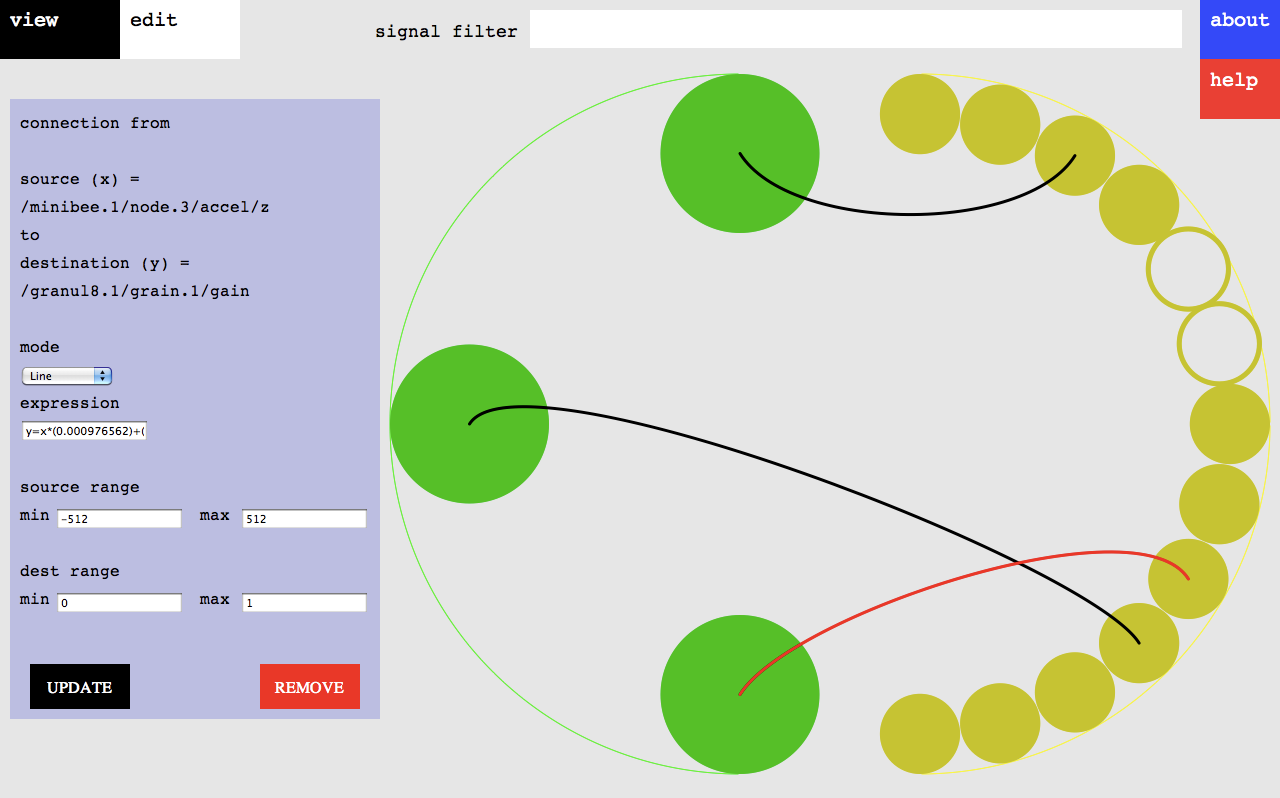
\includegraphics[width=0.88\textwidth]{vizmapperEight.png}
\caption{/source.3 branch of second level of output signals and first level of input signals in Vizmapper}
\label{fig:vizEight}
\end{figure}

\begin{figure}[p]
\centering
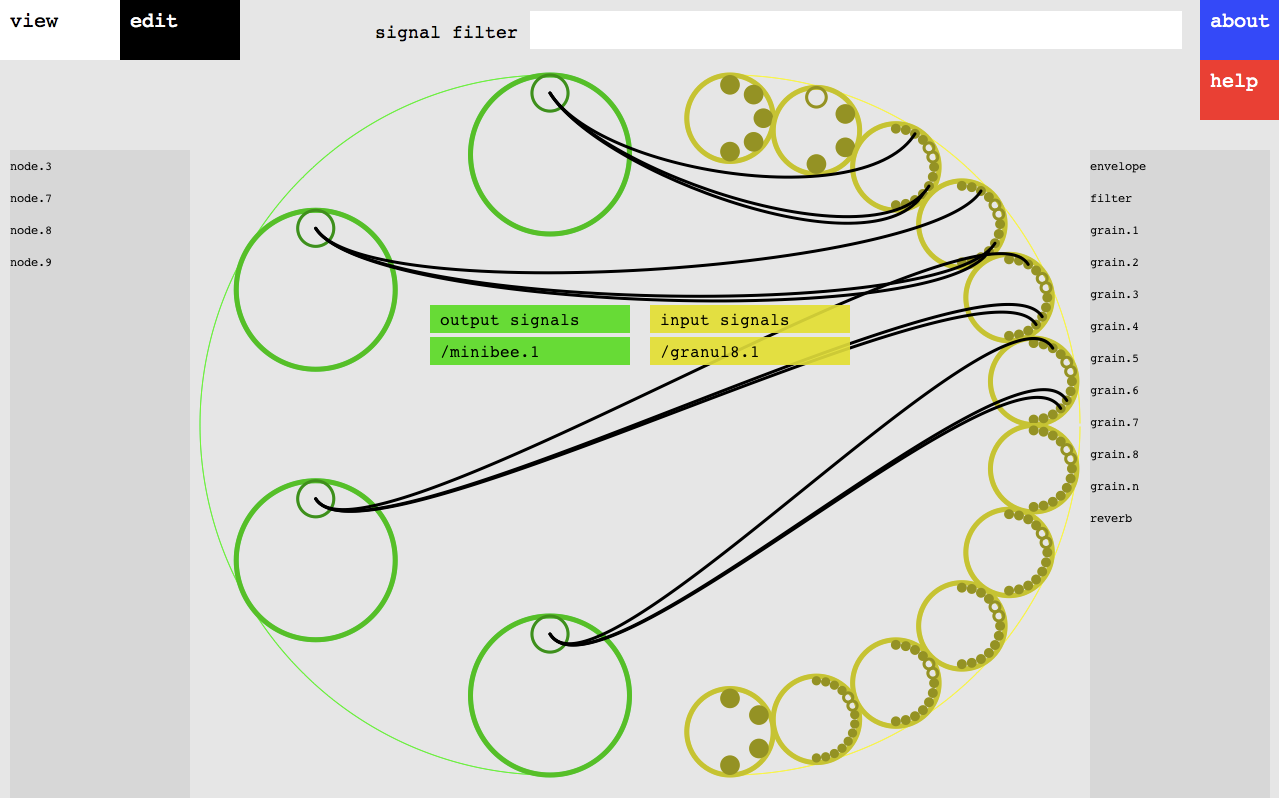
\includegraphics[width=0.88\textwidth]{vizmapperNine.png}
\caption{/source.3 branch of second level of output signals and /dest.3/synth1 branch of third level of input signals in Vizmapper}
\label{fig:vizNine}
\end{figure}

\begin{figure}[p]
\centering
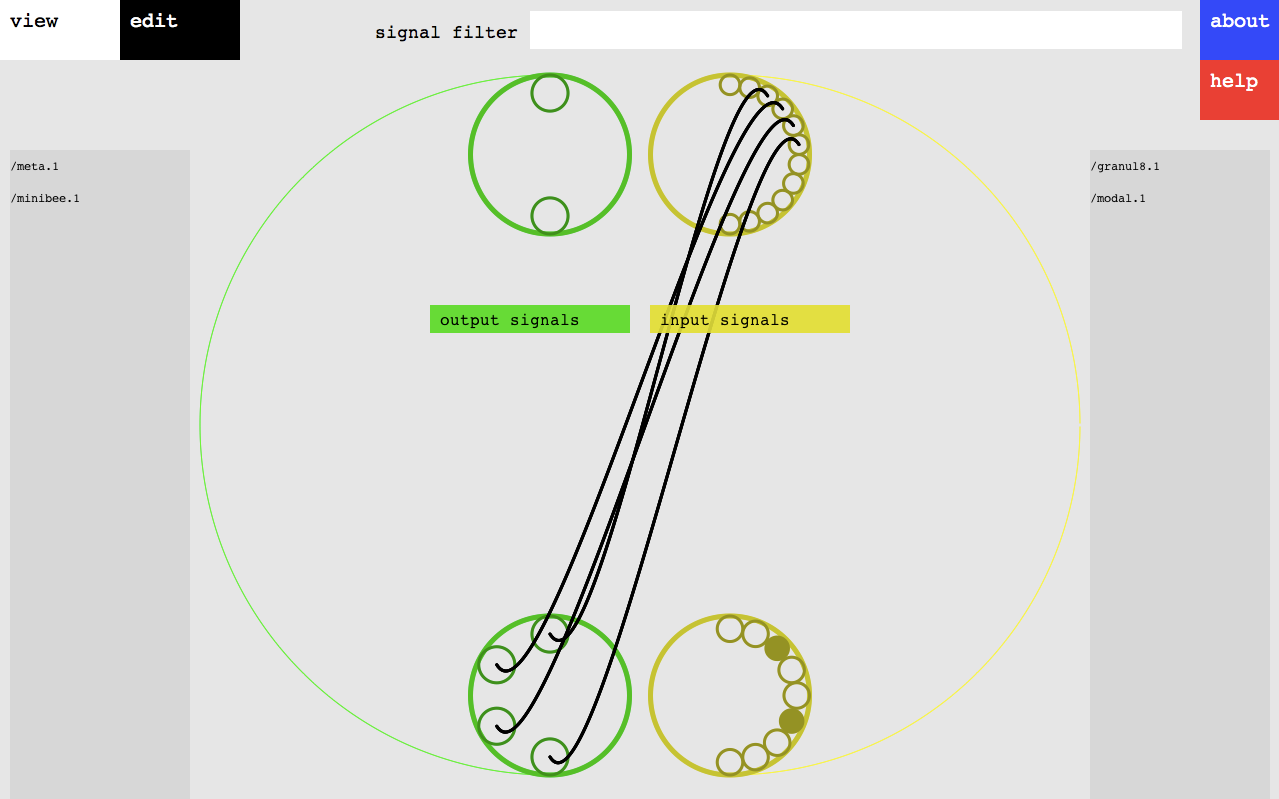
\includegraphics[width=0.88\textwidth]{vizmapperTen.png}
\caption{First level of output signals and first level of input signals in Vizmapper}
\label{fig:vizTen}
\end{figure}

\begin{figure}[p]
\centering
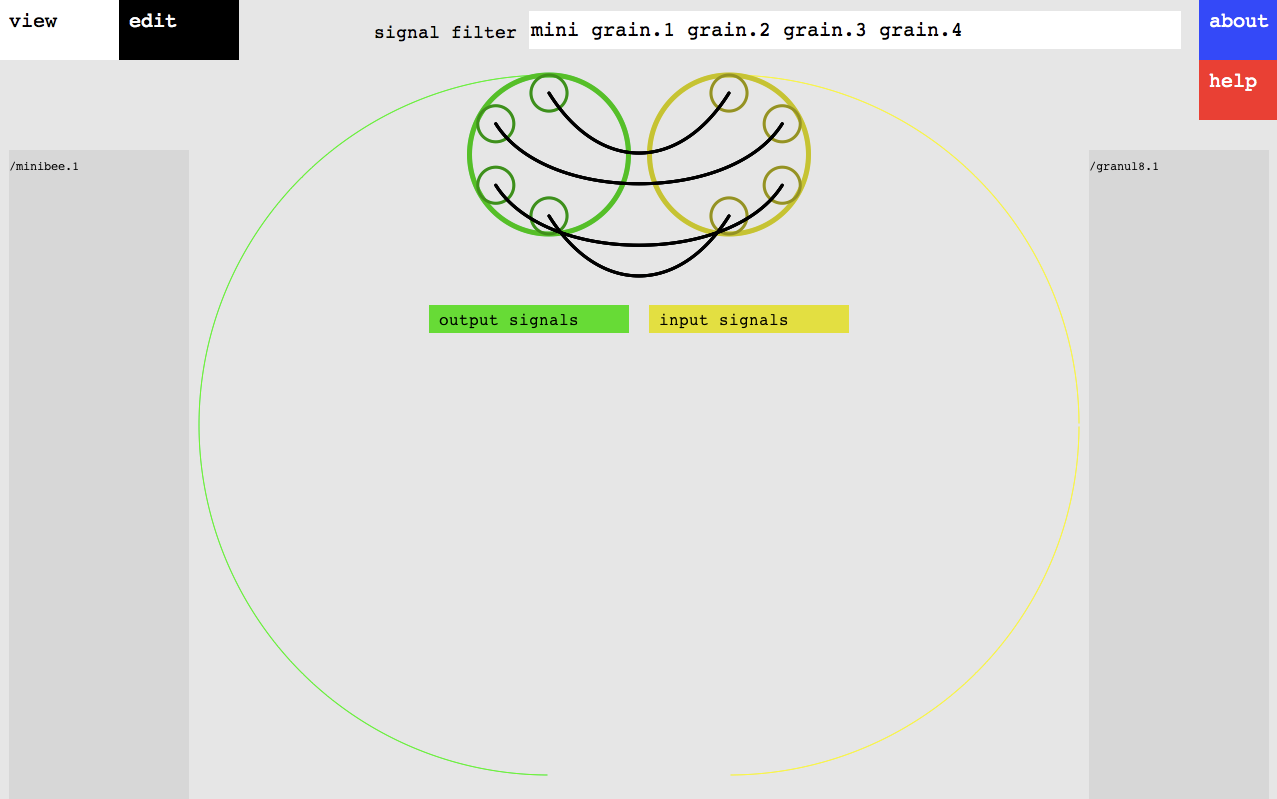
\includegraphics[width=0.88\textwidth]{vizmapperEleven.png}
\caption{/source.3 branch of second level of output signals and first level of input signals in Vizmapper}
\label{fig:vizEleven}
\end{figure}

\begin{figure}[htb]
\centering
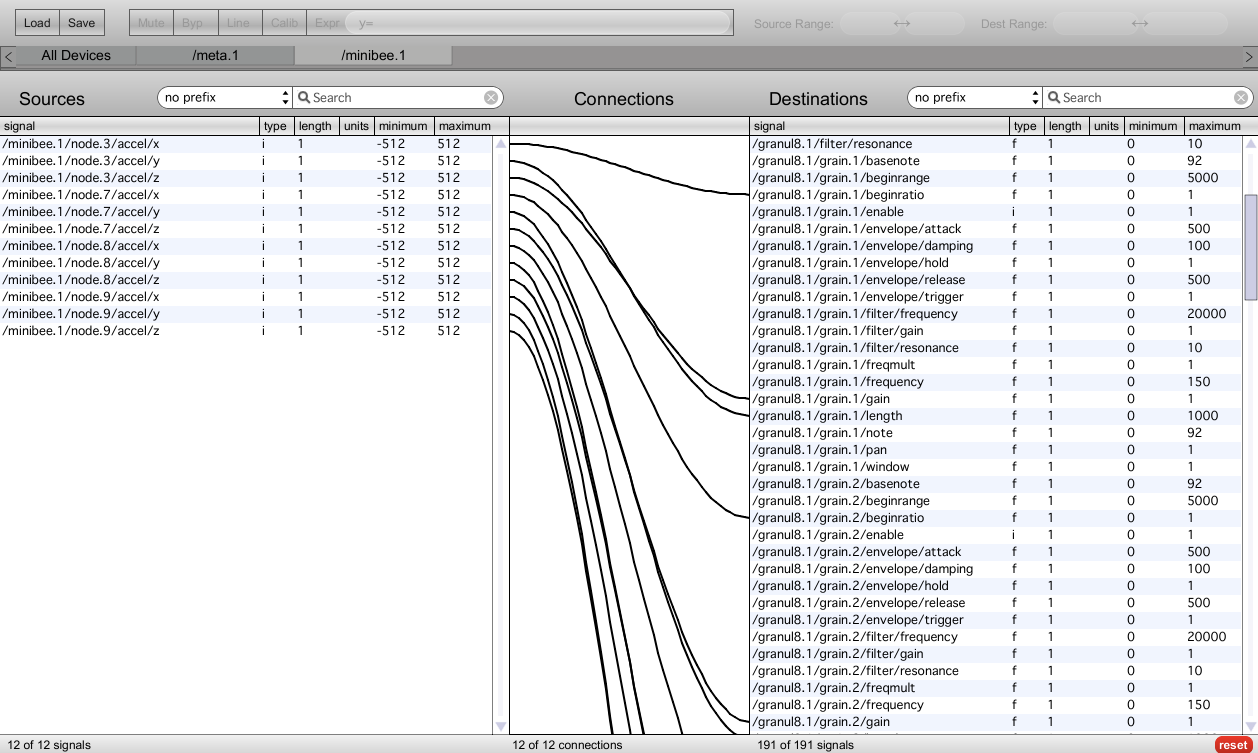
\includegraphics[width=0.88\textwidth]{maxmapperSecond.png}
\caption{/source.3 branch of second level of output signals and /dest.3/synth1 branch of third level of input signals in Vizmapper}
\label{fig:maxTwo}
\end{figure}

\section{Summary}

The Vizmapper interface provides all the functionality necessary to create a mapping on a Mapper network. The central argument is that through the process of understanding the mapping task and researching user interface design principles, data visualization principles, and human cognitive processes, this thesis research has resulted in an effective interface for configuring mappings that scales to a MSN with many signals.
